\documentclass[aspectratio=169,11pt]{beamer}
\usetheme{default}
\usecolortheme{default}

\setbeamertemplate{navigation symbols}{}
\setbeamertemplate{footline}[frame number]

\usepackage{amsmath}
\usepackage{booktabs}
\usepackage{graphicx}
\usepackage{tikz}
\usetikzlibrary{shapes,arrows,positioning,calc}

% Small citation macro
\newcommand{\citeslide}[1]{\hfill{\footnotesize [#1]}}

\title{Anisotropic Substrates for Reaction-Diffusion Computing}
\subtitle{Test 4: Design and Numerical Setup}
\author{Srivijayesh Venugopal}
\date{Cranfield IRP 2025-26 --- Supervisor Update, July 2026}

\begin{document}

% ---------------------------------------------------------------------
\begin{frame}
\titlepage
\end{frame}

% ---------------------------------------------------------------------
\begin{frame}{Why anisotropy?}

\textbf{Current substrate knobs are binary or scalar:}
\begin{itemize}
    \item Channel walls either \textbf{block} or \textbf{pass} a wave --- a binary, all-or-nothing weight.
    \item The light-suppression field $\phi(x,y)$ scales excitability, but isotropically.
\end{itemize}

\vspace{0.3cm}
\textbf{Anisotropic diffusion is a graded, direction-dependent weight:}
\begin{itemize}
    \item A diffusion tensor $D(x,y)$ slows waves along one axis and speeds them along another --- a \emph{continuous, directional} transfer function.
    \item Orientation and contrast can vary smoothly in space \textrightarrow{} trainable tensor fields.
\end{itemize}

\vspace{0.3cm}
\textbf{Novelty:} geometry and light fields are established knobs in excitable-media computing; \textbf{trained diffusion tensors are not.}
\citeslide{Steinbock et al., Science 1995; Keener, J.~Math.~Biol. 1991}

\end{frame}

% ---------------------------------------------------------------------
\begin{frame}{Physical realisations}

Anisotropic excitable media exist and are measurable:

\vspace{0.2cm}
\begin{itemize}
    \item \textbf{Aligned gels / fibres:} BZ reagents immobilised in aligned polymer networks or cellulose fibres --- diffusion is faster along the fibre axis.
    \item \textbf{Printed catalyst patterns:} stripes of catalyst printed on a substrate impose direction-dependent propagation \citeslide{Steinbock et al., Science 1995}.
    \item \textbf{Cardiac tissue:} the best-measured anisotropic excitable medium; fibre-aligned conduction with $D_\parallel / D_\perp \approx 4$--$9$.
    \item \textbf{Homogenised microstructure:} any periodic fine-scale layout (pillars, slits, pores) coarse-grains into an effective tensor $D(x,y)$ --- this is how a structured BZ reactor would acquire its anisotropy.
\end{itemize}

\vspace{0.3cm}
\centering
\textbf{So a trained tensor field is a design target that a real microstructured substrate could deliver.}

\end{frame}

% ---------------------------------------------------------------------
\begin{frame}{Governing equations}

Tyson--Fife Oregonator with tensor diffusion:
\begin{align*}
    \frac{\partial u}{\partial t} &= \frac{1}{\varepsilon}\left[ u - u^2 - (f v + \phi)\,\frac{u-q}{u+q} \right] + \nabla \cdot \left( D\, \nabla u \right) \\
    \frac{\partial v}{\partial t} &= u - v
\end{align*}

\vspace{0.2cm}
\begin{itemize}
    \item $D$ is a symmetric positive-definite tensor:
    \[
        D = \begin{pmatrix} D_{xx} & D_{xy} \\ D_{xy} & D_{yy} \end{pmatrix},
        \qquad
        D = R(\theta)
        \begin{pmatrix} D_\parallel & 0 \\ 0 & D_\perp \end{pmatrix}
        R(\theta)^{\mathsf T},
        \qquad r = \frac{D_\parallel}{D_\perp}.
    \]
    \item Principal axes rotated by $\theta$; contrast ratio $r$ is the anisotropy strength.
    \item Primary runs use \textbf{Barkley kinetics} ($a = 0.75$, $b = 0.01$, $\varepsilon = 0.02$) for speed; Oregonator runs provide chemical grounding.
\end{itemize}

\end{frame}

% ---------------------------------------------------------------------
\begin{frame}{Theory: what we expect}

Plane-wave speed in an excitable medium scales with diffusivity as
\[
    c \propto \sqrt{D}
\]
\citeslide{Keener, J.~Math.~Biol. 1991; Tyson \& Keener, Physica D 1988}

\vspace{0.3cm}
Two testable laws follow:

\begin{enumerate}
    \item \textbf{Ellipse law} --- a point-seeded target wave grows as an ellipse with axis speeds
    \[
        \frac{c_\parallel}{c_\perp} = \sqrt{r}.
    \]
    \item \textbf{Angular law} --- a plane wave propagating at angle $\theta$ to the fast axis travels at
    \[
        c(\theta) = \sqrt{c_\parallel^2 \cos^2\theta + c_\perp^2 \sin^2\theta}.
    \]
\end{enumerate}

\vspace{0.2cm}
\centering
\textbf{Test 4 checks these laws numerically, then uses orientation as a transfer knob.}

\end{frame}

% ---------------------------------------------------------------------
\begin{frame}{Numerical setup}

\begin{table}
\centering
\small
\begin{tabular}{p{4.6cm}p{8.2cm}}
\toprule
\textbf{Item} & \textbf{Choice} \\
\midrule
Grid & $256 \times 256$ (Tests 4a, 4b); channel-with-patch geometry (Test 4c) \\
Spacing / timestep & $DX = 1$; $DT = 0.05$ ($DT = 0.02$ for $r = 8$) \\
Time integration & Explicit FDM \\
Tensor diffusion & Divergence (flux) form with face-averaged tensors \\
Reaction terms & Operator splitting, adaptive reaction subcycling (analytic-Jacobian step control) \\
Boundaries & True no-flux (Neumann) walls \\
Failure handling & NaN tripwire, \textbf{no clipping} of state variables \\
\bottomrule
\end{tabular}
\end{table}

\vspace{0.3cm}
\textbf{Stability constraint} (explicit scheme, tensor diffusion):
\[
    DT \;\le\; \frac{DX^2}{4\,\lambda_{\max}(D)}
\]
\centering
$DT = 0.02$ at $r = 8$ keeps the diffusion number below the stability limit.

\end{frame}

% ---------------------------------------------------------------------
\begin{frame}{Tensor discretisation: flux form}

The diffusion term is discretised in conservative flux form. Face fluxes:
\[
    F_x = D_{xx}^{\,\text{face}}\, \frac{\partial u}{\partial x}
        + D_{xy}^{\,\text{face}}\, \frac{\partial u}{\partial y},
    \qquad
    \nabla \cdot (D \nabla u) \approx \frac{\partial F_x}{\partial x} + \frac{\partial F_y}{\partial y}.
\]

\vspace{0.2cm}
\begin{itemize}
    \item Cross derivative $\partial u / \partial y$ at a face uses a \textbf{4-point stencil} centred on the face.
    \item Tensor components at faces are \textbf{face-averaged} from neighbouring cells --- handles tensor discontinuities (e.g.\ patch boundaries) without smearing.
    \item The divergence of face fluxes is a standard centred difference \textrightarrow{} conservative, exact no-flux at walls.
\end{itemize}

\vspace{0.3cm}
\textbf{Sanity check:} for isotropic $D = D_u I$ the stencil reduces \emph{exactly} to the 5-point Laplacian --- verified to machine precision ($4 \times 10^{-16}$).

\end{frame}

% ---------------------------------------------------------------------
\begin{frame}{Parameter sets: two kinetic models}

\begin{table}
\centering
\small
\begin{tabular}{lcc}
\toprule
\textbf{Parameter} & \textbf{Barkley} & \textbf{Excitable Oregonator} \\
\midrule
$a$ / $f$      & $a = 0.75$        & $f = 1.4375$ \\
$b$ / $q$      & $b = 0.01$        & $q = 0.002$ \\
$\varepsilon$  & $0.02$            & $0.0501$ \\
$\phi$         & ---               & $0.010$ \\
$D_u$          & $1$               & $1$ \\
$D_v$          & $0$               & $0$ \\
Initial state  & rest $(0,0)$      & rest state $u^* = v^* = 0.0031$ \\
\bottomrule
\end{tabular}
\end{table}

\vspace{0.3cm}
\textbf{Why two models?}
\begin{itemize}
    \item \textbf{Barkley:} fast, clean headline measurements of the speed laws (cheap sweeps over $r$ and $\theta$).
    \item \textbf{Oregonator:} confirms the results carry over to the chemically grounded BZ kinetics.
\end{itemize}

\end{frame}

% ---------------------------------------------------------------------
\begin{frame}{Experiment 4a: target wave in a uniform anisotropic medium}

\begin{columns}
\begin{column}{0.55\textwidth}
\textbf{Setup:}
\begin{itemize}
    \item Point seed at the centre of a uniform medium with tensor $D$, $D_\perp = 1$.
    \item Sweep contrast $r \in \{1, 2, 4, 8\}$.
    \item Wavefront grows as an ellipse; measure the two axis speeds $c_\parallel$, $c_\perp$.
\end{itemize}

\vspace{0.3cm}
\textbf{Success criterion:}
\[
    \left| \frac{c_\parallel / c_\perp}{\sqrt{r}} - 1 \right| \le 10\%.
\]

\vspace{0.2cm}
Validates both the tensor discretisation and the $\sqrt{D}$ scaling law.
\end{column}

\begin{column}{0.40\textwidth}
\centering
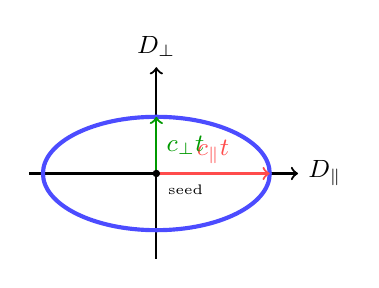
\begin{tikzpicture}[scale=0.9]
% fast axis
\draw[->, thick] (-1.8,0) -- (2.0,0) node[right] {\small $D_\parallel$};
\draw[->, thick] (0,-1.2) -- (0,1.5) node[above] {\small $D_\perp$};
% ellipse wavefront
\draw[blue!70, line width=1.5pt] (0,0) ellipse (1.6 and 0.8);
% semi-axes
\draw[red!70, thick, ->] (0,0) -- (1.6,0) node[midway, above] {\small $c_\parallel t$};
\draw[green!60!black, thick, ->] (0,0) -- (0,0.8) node[midway, right] {\small $c_\perp t$};
% seed
\fill[black] (0,0) circle (1.5pt) node[below right=1pt] {\tiny seed};
\end{tikzpicture}

\vspace{0.1cm}
{\footnotesize Elliptical target wave; axis ratio $\approx \sqrt{r}$.}
\end{column}
\end{columns}

\end{frame}

% ---------------------------------------------------------------------
\begin{frame}{Experiment 4b: plane wave at an angle to the fast axis}

\begin{columns}
\begin{column}{0.55\textwidth}
\textbf{Setup:}
\begin{itemize}
    \item Fix $r$; tilt the \emph{tensor} by $\theta \in \{0^\circ, 30^\circ, 45^\circ, 60^\circ, 90^\circ\}$.
    \item Wave is always seeded as an $x$-propagating plane wave --- only the substrate rotates, keeping the measurement protocol identical across angles.
    \item Measure $c(\theta)$ and compare against the theory curve
    \[
        c(\theta) = \sqrt{c_\parallel^2 \cos^2\theta + c_\perp^2 \sin^2\theta}.
    \]
\end{itemize}
\end{column}

\begin{column}{0.40\textwidth}
\centering
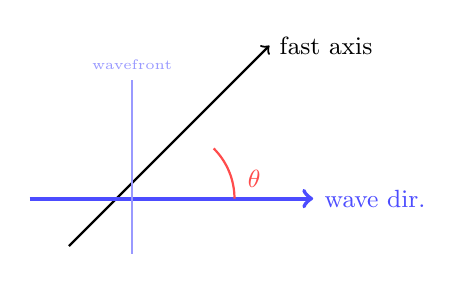
\begin{tikzpicture}[scale=1.0]
% tilted fast axis
\draw[->, thick, rotate=45] (-1.7,0) -- (1.9,0) node[right, rotate=0] {\small fast axis};
% horizontal wave direction
\draw[->, blue!70, line width=1.5pt] (-1.7,-0.6) -- (1.9,-0.6) node[right] {\small wave dir.};
% angle arc
\draw[red!70, thick] (0.9,-0.6) arc[start angle=0, end angle=45, radius=0.9];
\node[red!70] at (1.15,-0.35) {\small $\theta$};
% plane wavefront
\draw[blue!40, line width=1pt] (-0.4,-1.3) -- (-0.4,0.9);
\node[blue!40] at (-0.4,1.1) {\tiny wavefront};
\end{tikzpicture}

\vspace{0.1cm}
{\footnotesize Tensor tilted by $\theta$; wave kept $x$-propagating.}
\end{column}
\end{columns}

\end{frame}

% ---------------------------------------------------------------------
\begin{frame}{Experiment 4c: channel through an anisotropic patch}

\begin{columns}
\begin{column}{0.55\textwidth}
\textbf{Setup:}
\begin{itemize}
    \item A channel of isotropic medium ($D = 1$) passes through a rectangular patch with $r = 4$, $D_\perp = 1$ inside; isotropic outside.
    \item Rotate the patch orientation $\theta$ relative to the channel axis.
    \item Measure the \textbf{transmission delay} of a pulse crossing the patch as a function of $\theta$.
\end{itemize}

\vspace{0.3cm}
\textbf{Question:} does patch orientation act as a \textbf{continuously tunable transfer knob} --- a graded delay/gain element for wave-based computing?
\end{column}

\begin{column}{0.40\textwidth}
\centering
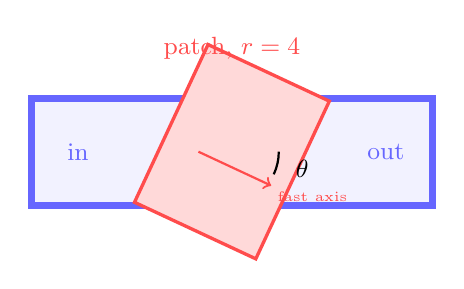
\begin{tikzpicture}[scale=0.85]
% channel
\draw[draw=blue!60, line width=2.5pt, fill=blue!5] (0,0) rectangle (6,1.6);
% tilted patch
\draw[draw=red!70, line width=1.2pt, fill=red!15, rotate around={-25:(3,0.8)}] (2.0,-0.5) rectangle (4.0,2.1);
% labels
\node[blue!60] at (0.7,0.8) {\small in};
\node[blue!60] at (5.3,0.8) {\small out};
\node[red!70] at (3,2.35) {\small patch, $r=4$};
% fast axis arrow inside patch
\draw[->, thick, red!70] (2.5,0.8) -- ($(2.5,0.8)+(-25:1.2)$) node[below right=-2pt] {\tiny fast axis};
% theta arc
\draw[black, thick] (3.7,0.8) arc[start angle=0, end angle=-25, radius=0.8];
\node at (4.05,0.55) {\small $\theta$};
\end{tikzpicture}

\vspace{0.1cm}
{\footnotesize Channel (isotropic) crossing a tilted anisotropic patch.}
\end{column}
\end{columns}

\end{frame}

% ---------------------------------------------------------------------
\begin{frame}{Verification and controls}

\begin{itemize}
    \item \textbf{No-stimulus control:} an unseeded domain must remain at rest for the full run --- catches spurious excitation from the tensor stencil or boundaries.
    \item \textbf{Rest-state initialisation:} with $\phi > 0$ the true rest state is $u^* = v^* = 0.0031$, \textbf{not} $(0,0)$; initialising at $(0,0)$ would itself be a perturbation.
    \item \textbf{Isotropy reduction:} flux-form stencil reduces exactly to the 5-point Laplacian (verified to $4\times10^{-16}$).
    \item \textbf{Convergence harness:} grid/timestep refinement harness exists ---
    \begin{itemize}
        \item temporal (halving $DT$): measured error $\le 1.5\%$ on wave speed;
        \item spatial (halving $DX$): reported as an explicit error bar on every speed measurement.
    \end{itemize}
    \item \textbf{NaN tripwire, no clipping:} any instability aborts the run rather than silently corrupting results.
\end{itemize}

\end{frame}

% ---------------------------------------------------------------------
\begin{frame}{What success looks like / next steps}

\textbf{If the $\sqrt{r}$ ellipse law and the angular law verify:}
\begin{itemize}
    \item Anisotropy becomes a \textbf{certified design knob} --- the speed ratio is predictable from $D$ alone.
    \item Next: \textbf{trained orientation fields} $\theta(x,y)$ --- optimise a spatially varying tensor so that input pulses are steered/delayed to hit a target readout, extending the geometry-training loop to tensor fields.
\end{itemize}

\vspace{0.4cm}
\textbf{Status of Test 4 runs:}
\begin{itemize}
    \item 4a (ellipse law) --- [results pending --- next meeting]
    \item 4b (angular law) --- [results pending --- next meeting]
    \item 4c (patch transmission) --- [results pending --- next meeting]
\end{itemize}

\vspace{0.3cm}
\centering
\textbf{Setup is complete and verified; measurements are being finalised.}

\end{frame}

% ---------------------------------------------------------------------
\begin{frame}{References}

{\footnotesize
\begin{enumerate}
    \item O. Steinbock, P. Kettunen \& K. Showalter. Anisotropy and spiral organizing centers in patterned excitable media. \textit{Science} 269, 1857--1860 (1995).
    \item J. P. Keener. The effects of discrete gap junction coupling on propagation in myocardium. \textit{J.~Math.~Biol.} 29, 49--82 (1991).
    \item J. J. Tyson \& J. P. Keener. Singular perturbation theory of traveling waves in excitable media. \textit{Physica D} 32, 327--361 (1988).
    \item J. J. Tyson \& P. C. Fife. Target patterns in a realistic model of the Belousov--Zhabotinskii reaction. \textit{J.~Chem.~Phys.} 73, 2224 (1980).
    \item D. Barkley. A model for fast computer simulation of waves in excitable media. \textit{Physica D} 49, 61--70 (1991).
    \item A. Adamatzky \& B. De Lacy Costello. Experimental logical gates in a reaction-diffusion medium. \textit{Phys. Rev. E} 66, 046112 (2002).
\end{enumerate}
}

\end{frame}

\end{document}
